\documentclass[10pt]{article}
\listfiles               %  print all files needed to compile this document

\usepackage{amsmath}
\usepackage{listings}
\usepackage{xparse}
%\usepackage{color}
\usepackage{xcolor}
\usepackage{graphicx}
\usepackage{dcolumn}
\usepackage{bm}
\usepackage[colorlinks=true,urlcolor=blue,citecolor=blue]{hyperref}
\usepackage{color}
%\usepackage{physics}
\usepackage{algorithm2e}
\usepackage{algpseudocode}
\usepackage{pgfplots}
\usepackage{pgfplotstable, booktabs, mathpazo}
\usepackage{natbib}

\pgfplotsset{compat=1.15}
\lstset{%
frame=single,
xleftmargin=.25in,
language=,
breaklines=true,
}

%\pgfplotstableset{
%    every head row/.style={before row=\toprule \hline ,after row=\hline\hline \midrule},
%    every last row/.style={after row=\hline \bottomrule},
%    every first column/.style={
%        column type/.add={|}{}
%        },
%    every last column/.style={
%        column type/.add={}{|}
%        },
%}
\pgfplotstableset{%
every head row/.style={before row=\toprule \toprule, after row=\midrule \midrule},
every last row/.style={after row=\bottomrule \bottomrule}
}

%\begin{figure}[hbtp]
%\includegraphics[scale=0.4]{.pdf}
%\caption{}
%\label{fig:}
%\end{figure}

%\begin{tikzpicture}
%    \begin{axis}[
%            title= Earth-Sun system, Forward Euler integration,
%            xlabel={$x$},
%            ylabel={$y$},
%        ]
%        \addplot table {../runresults/earthEuler2body.dat}
%    \end{axis}
%\end{tikzpicture}

%=============================================================================================================
% When writing, all code calls and similar have been placed in separate .txt files, so as to ease change and
% reference for later. Change input in one of the related files and recompile to update.
% to compile:
% $ ~/latexrun/latexrun report.tex
% latexrun github: https://github.com/aclements/latexrun
% Then open with your favourite pdf reader.
%=============================================================================================================

\begin{document}

\title{%
Report of setup of Variscite
\large
VAR-SOM-MX6 Yocto Sumo release
}

\author{Anders Gjolme Eriksen}
\maketitle

\begin{figure*}[hbtp]
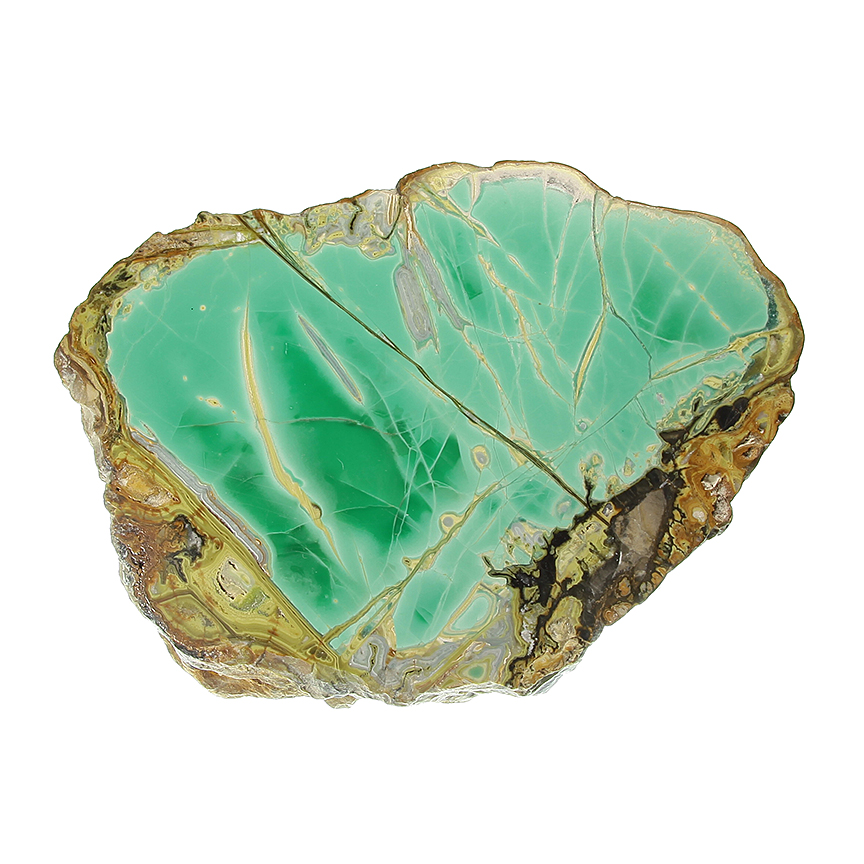
\includegraphics[scale=0.4]{./variscite.jpg}
\end{figure*}

\tableofcontents
\newpage

\section{introduction}

The \href{http://variwiki.com/index.php?title=VAR-SOM-MX6\_Yocto\&release=RELEASE\_SUMO\_V1.1\_VAR-SOM-MX6}{VAR-SOM-MX6 Yocto Sumo release from Variscite}
has a guide to follow for installation, but in previous and current releases have not been trivial to follow. The aim of here is to clarify the
methods and to provide the necessary corrections made.

Compilation info in ``.tex'' file. At the top, between the ``\%==\ldots'' signs.

\subsection{setup}

The recommended first reading is largely unneded. At time of writing, it is unavailable. In addition, there is no ``beginners guide''
to the Yocto release for VAR-SOM-MX6 that

%=========
Note: When initializing, the variviki does not list the folder ``build\_x11``. This will generally need to be added. This should be mentioned at relevant
points, but in case one slips through, it is worth noting. Another frequent issue, is when running programs from current folder, there is a need
to insert ''./'' infront of the path.
%========


%===========================================================================================================
\section{VAR-SOM-MX6 Yocto Sumo 2.5 based on FSL Community BSP 2.5 with 4.9.88\_2.0.0-ga Linux release}
Information found on \href{http://variwiki.com/index.php?title=Yocto\_Build\_Release&release=RELEASE\_SUMO\_V1.1\_VAR-SOM-MX6}{variwiki under Yocto Sumo release guide.}
website

\subsection{build x11 GUI demo image}
The given commands throw an error with setup-environment. Adding a ''./'' as below works. Next is building the demo image using bitbake, excluding QT content.
%-----------------
\lstinputlisting{./inputs/sourceYocto/demoGUI.txt}
%-----------------
Output in Appendix~\ref{app:GUIImage}.


%--------------------------------------------------------------
\subsection{console-only demo image}
Not built.\ Should not pose new issue beyond the GUI.\ GUI image is enough.

\subsection{Local conf customization}

\subsubsection{Change download directory.}
It is implied already being in directory ``/home/user/var-fslc-yocto/'' at execution.
Make and set permision for a yocto download file:

Change download path for the configuration file for yocto's build\_x11 setup $\rightarrow$ the given link does not work. You need to add the directory for the
build, making the addition~./build\_x11/conf/local.conf.
%-----------------
\lstinputlisting{./inputs/sourceYocto/downloadDir.txt}
%-----------------

\subsubsection{BuildResults}
The resulting files should be located in:  ``tmp/deploy/images/var-som-mx6'' Table layout of files on
\href{http://variwiki.com/index.php?title=Yocto_Build_Release&release=RELEASE_SUMO_V1.1_VAR-SOM-MX6#Build_Results}{web page}

%--------------------------------------------------------------
\subsection{create bootable SD card}

\subsubsection{SD structure.\ map of SD card structure after partitioning.}
schematics on the \href{http://variwiki.com/index.php?title=Yocto_Build_Release&release=RELEASE_SUMO_V1.1_VAR-SOM-MX6#SD_card_structure}{wiki}.

\subsubsection{Yocto pre-built}
The standard partition is not sensitive to SD size, nor does it include the install scripts. At time of writing, utilized extended version

Replace ``sdX'' with the right device name. This can be obtained by ``dmesg'' or ``lsusb'' or ``ls /dev/sd*'' command on your host Linux PC,
after the SD card reader is inserted.
Also notable, the partition containing the root file system is not named ``rootfs'' making for GUI and QT.\
\lstinputlisting{inputs/sourceYocto/prebuiltYocto.text}

\subsubsection{Create extended SD card}
This is a variscite partition shell script ``var-create-yocto-sdcard.sh'' which partitions the card and installs necessary files for NAND flash.

An issue that popped up, was the bash ``rename'' command.\ running a ``sudo apt-get install rename'' fixed issue.
(Replace /dev/sdX with your actual device, running ``dmesg'' will give you the relevant mount directory)
\lstinputlisting{inputs/sourceYocto/SDCard.txt}
Current run with fully partitioning SD card using option ``-a''

output in Appendix~\ref{app:extendedSDcard}

\subsection{Boot board through SD card}
images and directions per board fonud on
\href{http://variwiki.com/index.php?title=Yocto_Build_Release&release=RELEASE_SUMO_V1.1_VAR-SOM-MX6#Boot_the_board_with_a_bootable_SD_card}{wiki}

\subsubsection{Setting boot mode. 6.1.1 har instructions for MX6 custom board.}

\subsubsection{Automatic device tree selection in U-boot. Default enabled.}

\subsection{Flash images to NAND}
See Section~\ref{sect:NANDFlash}.


%===========================================================================================================
\section{Yocto NAND Flash Burning\label{sect:NANDFlash}}
\subsection{Introduction}
VAR-SOM-MX6 boots from on-SOM NAND flash. U-boot, kernel image and device tree blob are also stored in NAND flash.\
full recipee on \href{http://variwiki.com/index.php?title=Yocto_NAND_Flash_Burning&release=RELEASE_SUMO_V1.1_VAR-SOM-MX6}{wiki}

\subsection{NAND flash structure}
defined MTD partitions on NAND flash:
%-----------------
\lstinputlisting{./outputs/sourceYocto/relevantPartitionInfo.txt}
%-----------------
\subsection{eMMC structure}
Not explored.

\subsection{Yocto built binaries for NAND flash}
Images generated for NAND flash are located in ``tmp/deploy/images/var-som-mx6''. There is a table showing the expected files on the
\href{http://variwiki.com/index.php?title=Yocto\_NAND\_Flash\_Burning&release=RELEASE\_SUMO\_V1.1\_VAR-SOM-MX6#Yocto\_Built\_binaries\_for\_NAND\_flash\_.2F\_eMMC}{variwiki site}

\subsection{installing Yocto binaries}
If followed extended SD card creation, NAND flash scripts are already included on the SD card.

\subsubsection{images location}
\lstinputlisting{./outputs/sourceYocto/imageLocations.txt}

\subsubsection{Preparing images for NAND flash}
Note: the extended SD card creation makes these steps redundant.
The SD card should be mounted on the host computer. Assumed mount directory is ``/media/rootfs/''. If mounted into another folder, modify accordingly.\

setup:
%-----------------
\lstinputlisting{./inputs/imagePrepNANDFlash/setup.txt}
%-----------------
Linux:
%-----------------
\lstinputlisting{./inputs/imagePrepNANDFlash/linux.txt}
%-----------------
Device tree:
%-----------------
\lstinputlisting{./inputs/imagePrepNANDFlash/deviceTree.txt}
%-----------------
NAND images:
%-----------------
\lstinputlisting{./inputs/imagePrepNANDFlash/NANDImages.txt}
%-----------------

Other images on wiki.

\subsection{installing Yocto binaries}
When accessing board on linux, minicom needed to disable flow control in order to make any input.

%-----------------------------------------------------------
\subsubsection{Images locations}
directory structure on SD card
%-----------------
\lstinputlisting{./outputs/sourceYocto/directoryStructure.txt}
%-----------------

%=========================================================================================================
Further on would be to flash images and the like onto the board, but this is not a priority at this moment.
The main goal now is to get the toolchain up and running.
%=========================================================================================================


%=========================================================================================================
\section{Yocto toolchain installation for out of Yocto builds}
\subsection{prerequisits}
A full Yocto OpenEmbedded environment to generate the toolchain. This means following steps 1 and 3 from the guide to
\href{http://variwiki.com/index.php?title=Yocto\_Build\_Release&release=RELEASE\_SUMO\_V1.1\_VAR-SOM-MX6}{building yocto from source code}.


\subsection{Build toolchain}%============== redo layout!
run the following code, where the text from the wiki: setup-environment is replaced by~./setup-environment:
%-----------------
\lstinputlisting{./inputs/toolChain/build.txt}
%-----------------
Output can be found in Appendix~\ref{app:bitbakeToolChainIDESupport}
Then run the Tool chain build, output at~\ref{app:toolChainBuild}

\subsection{Build complete SDK}
build development environment with the required libraries in addition to the basic toolchain.
%lstinputlisting{inputs/toolChain/buildSDK.txt}
runoutput in Appendix~\ref{app:toolchainSDK}
Output will be located in tmp/deploy/sdk/.

\subsubsection{Install toolchain/SDK}
Installation is done with
\lstinputlisting{./inputs/toolChain/toolchainInstall.txt}
Returning:
\lstinputlisting{./outputs/toolChain/toolChainInstall.txt}

\subsection{Use of toolchain/SDK}
\lstinputlisting{./inputs/toolChain/toolchainLaunch.txt}

\newpage
\section{appendix}
Percentage completion of runs demarkated in ``\#'' signs. They do not follow the linebreak convention.
They do not follow the linebreak convention.\ there is not meaningful information in these lines. They
are included in order to stay true to results.

\subsection{bitbake of fslc image}
%-----------------
\lstinputlisting{./outputs/sourceYocto/bitbake_image_output.txt}\label{app:GUIImage}
%-----------------

\subsection{bitbake of toolchain}
outputh from build of IDE support:
%-----------------
\lstinputlisting{./outputs/toolChain/bitbakeMetaIdeSupport.txt}\label{app:toolChainIDESupport}
%-----------------
output from toolchain build:
%-----------------
\lstinputlisting{./outputs/toolChain/bitbakeToolChain.txt}\label{app:toolChainBuild}
%-----------------
\subsubsection{bild SDK}
%-----------------
\lstinputlisting{./outputs/toolChain/bitbakeSDKBuild.txt}\label{app:toolChainSDK}
%-----------------

%\bibliography{FULL PATH TO BIBLIOGRAPHY}
\end{document}
